% Chapter Template

\chapter{FDTD - Two-Dimensional Scenario} % Main chapter title

\label{Chapter3} % Change X to a consecutive number; for referencing this chapter elsewhere, use \ref{ChapterX}

%----------------------------------------------------------------------------------------
%	SECTION 1
%----------------------------------------------------------------------------------------

\section{Main Section 1}

%-----------------------------------
%	SUBSECTION 1
%-----------------------------------
\subsection{Subsection 1}
%-----------------------------------
%	SUBSECTION 2
%-----------------------------------

\subsection{Subsection 2}
%----------------------------------------------------------------------------------------
%	SECTION 2
%----------------------------------------------------------------------------------------

\section{C++ Implementation}

\section{Data Visualization}

\begin{figure}
	\centering
    \begin{subfigure}{.49\textwidth}
    	\centering
    	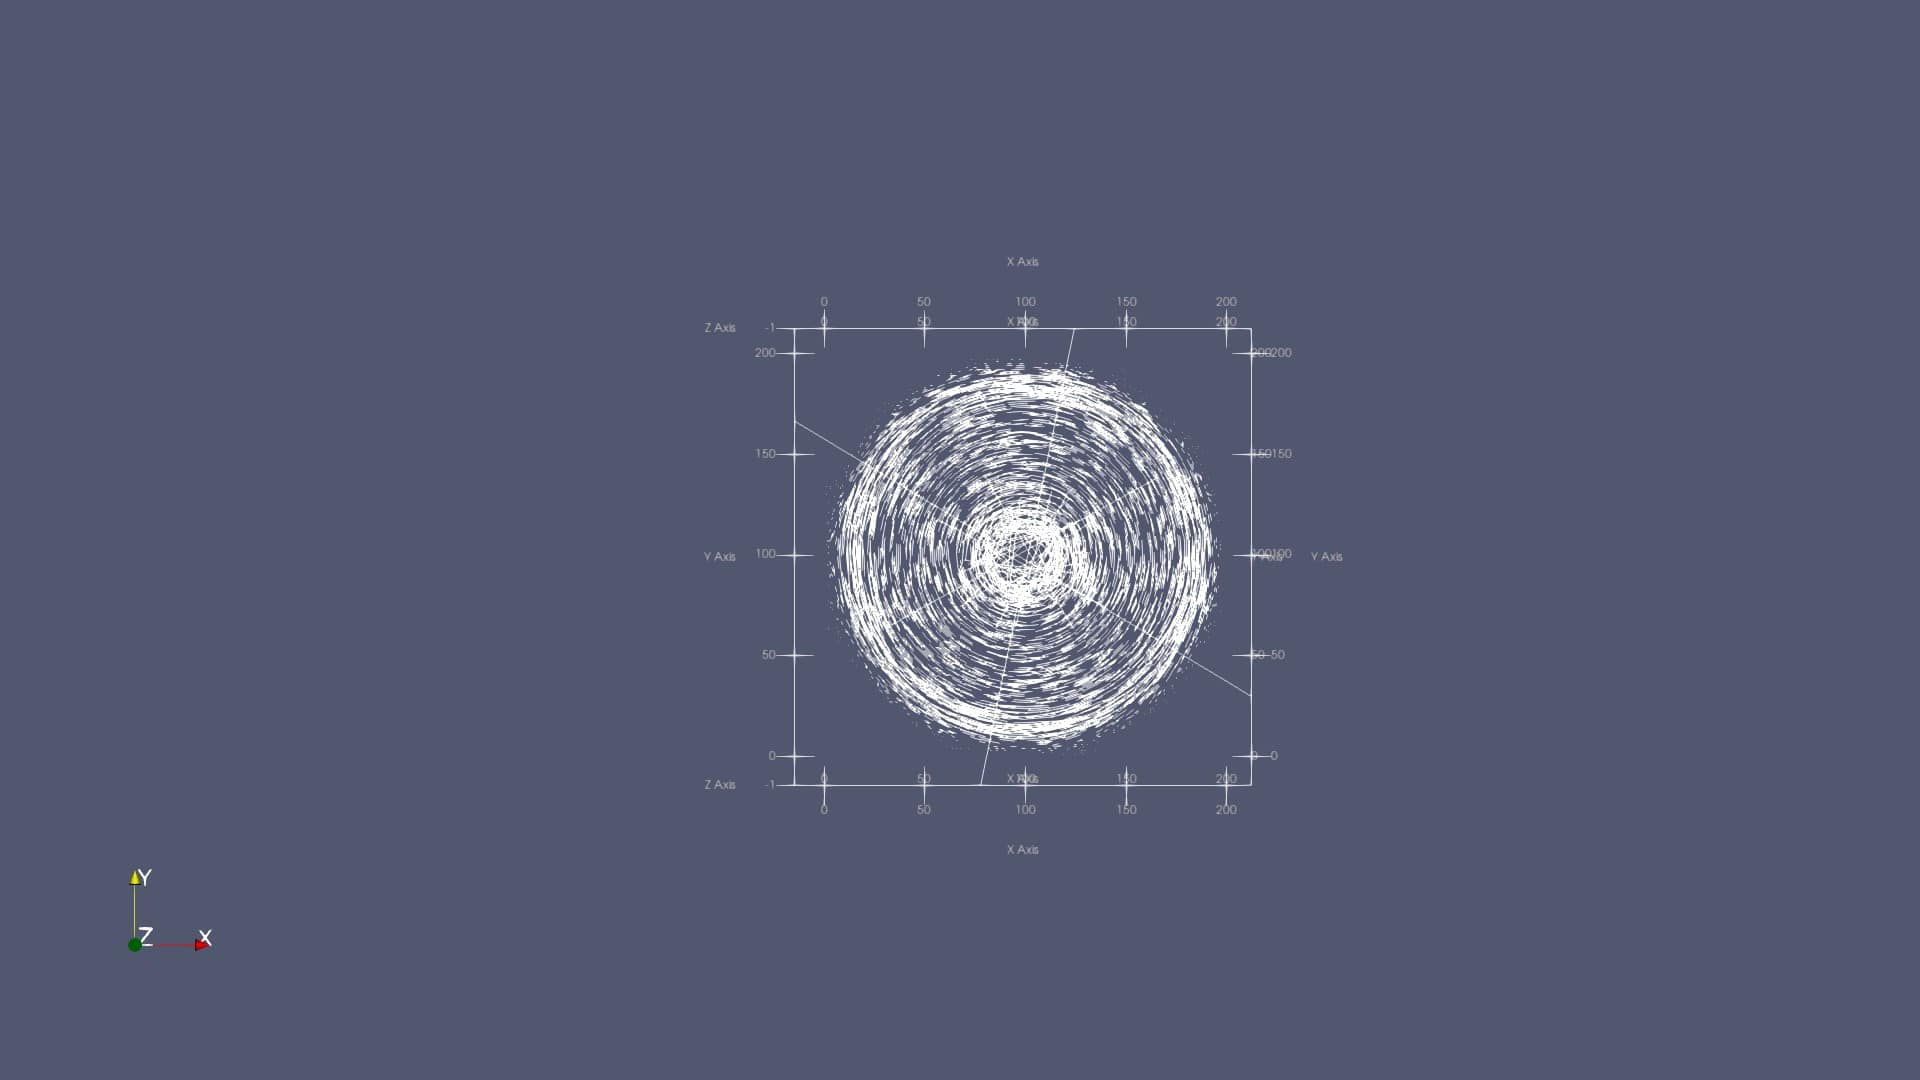
\includegraphics[width=.95\linewidth]{Figures/FDTD2DE1}
    	\caption{t = 200}
    \end{subfigure}
    \begin{subfigure}{.49\textwidth}
    	\centering
    	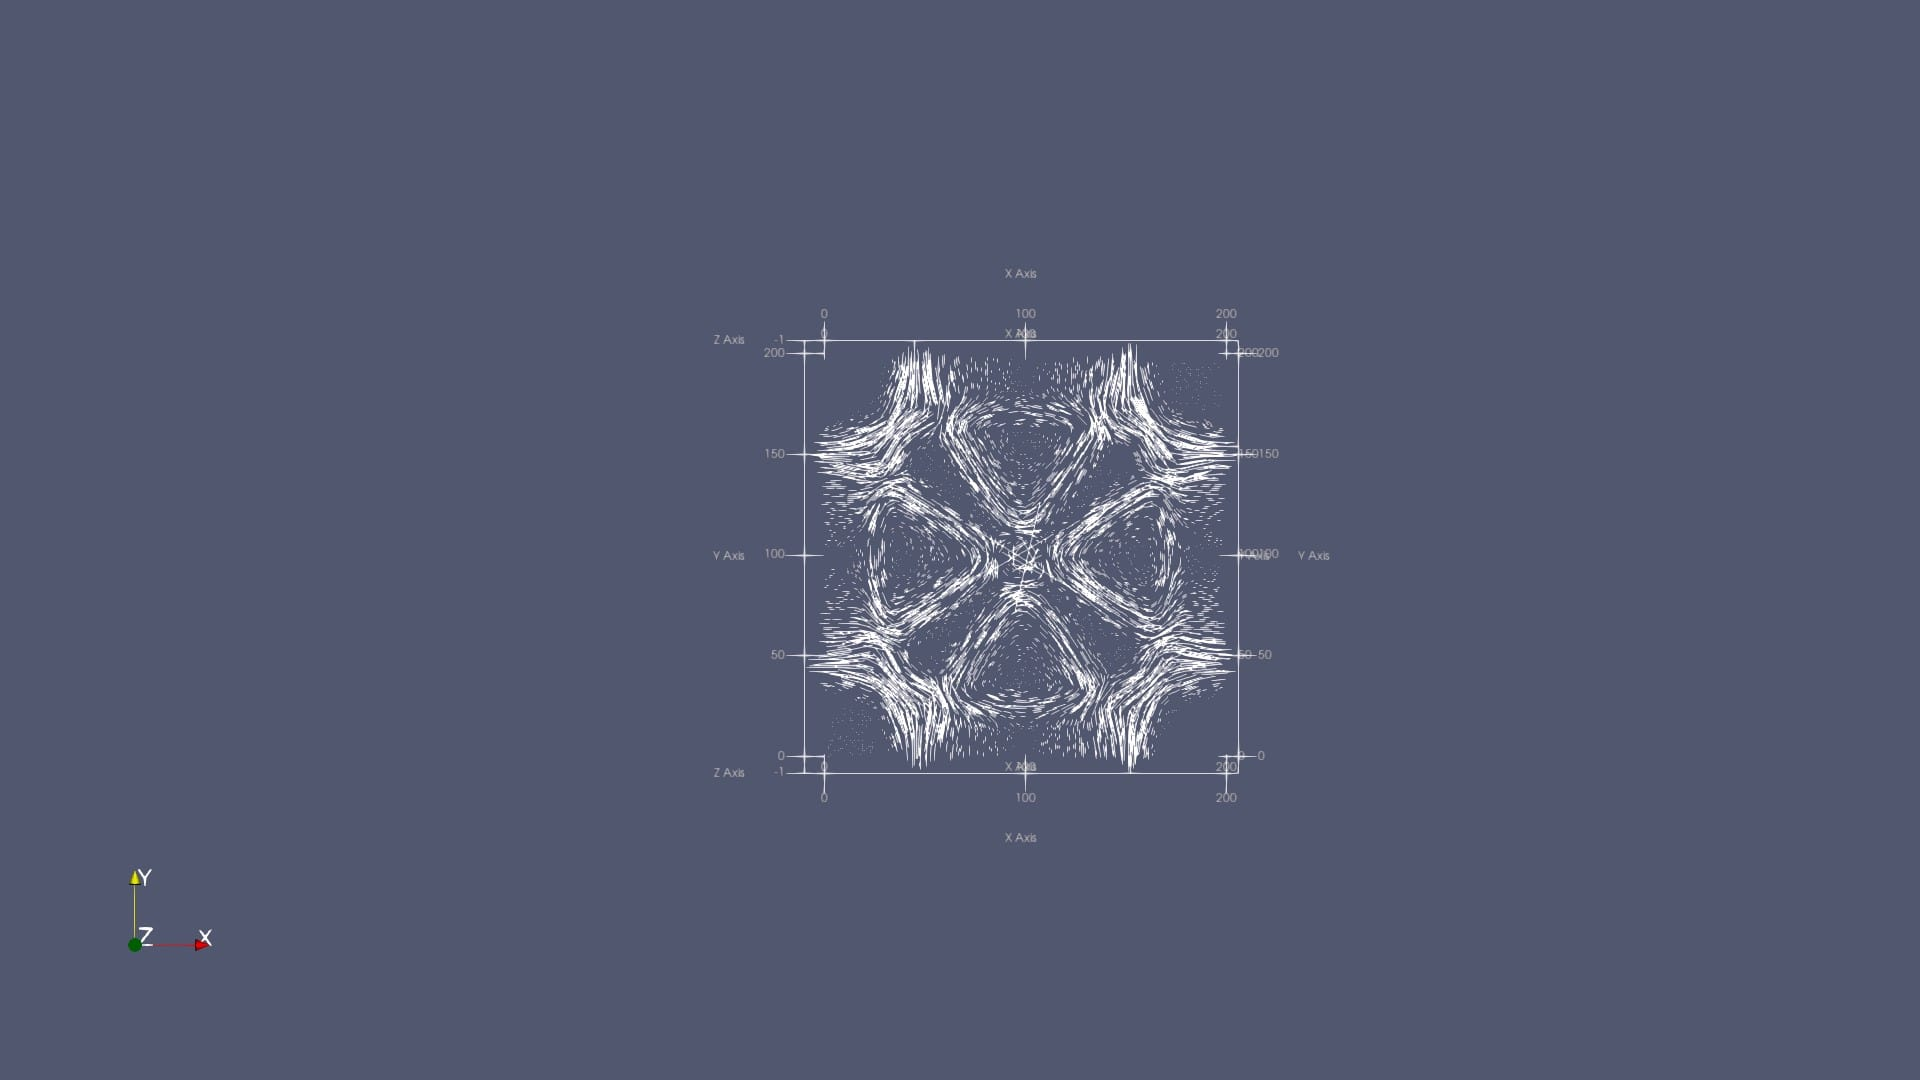
\includegraphics[width=.95\linewidth]{Figures/FDTD2DE2}
    	\caption{t = 400}
    \end{subfigure}
    \begin{subfigure}{.49\textwidth}
    	\centering
    	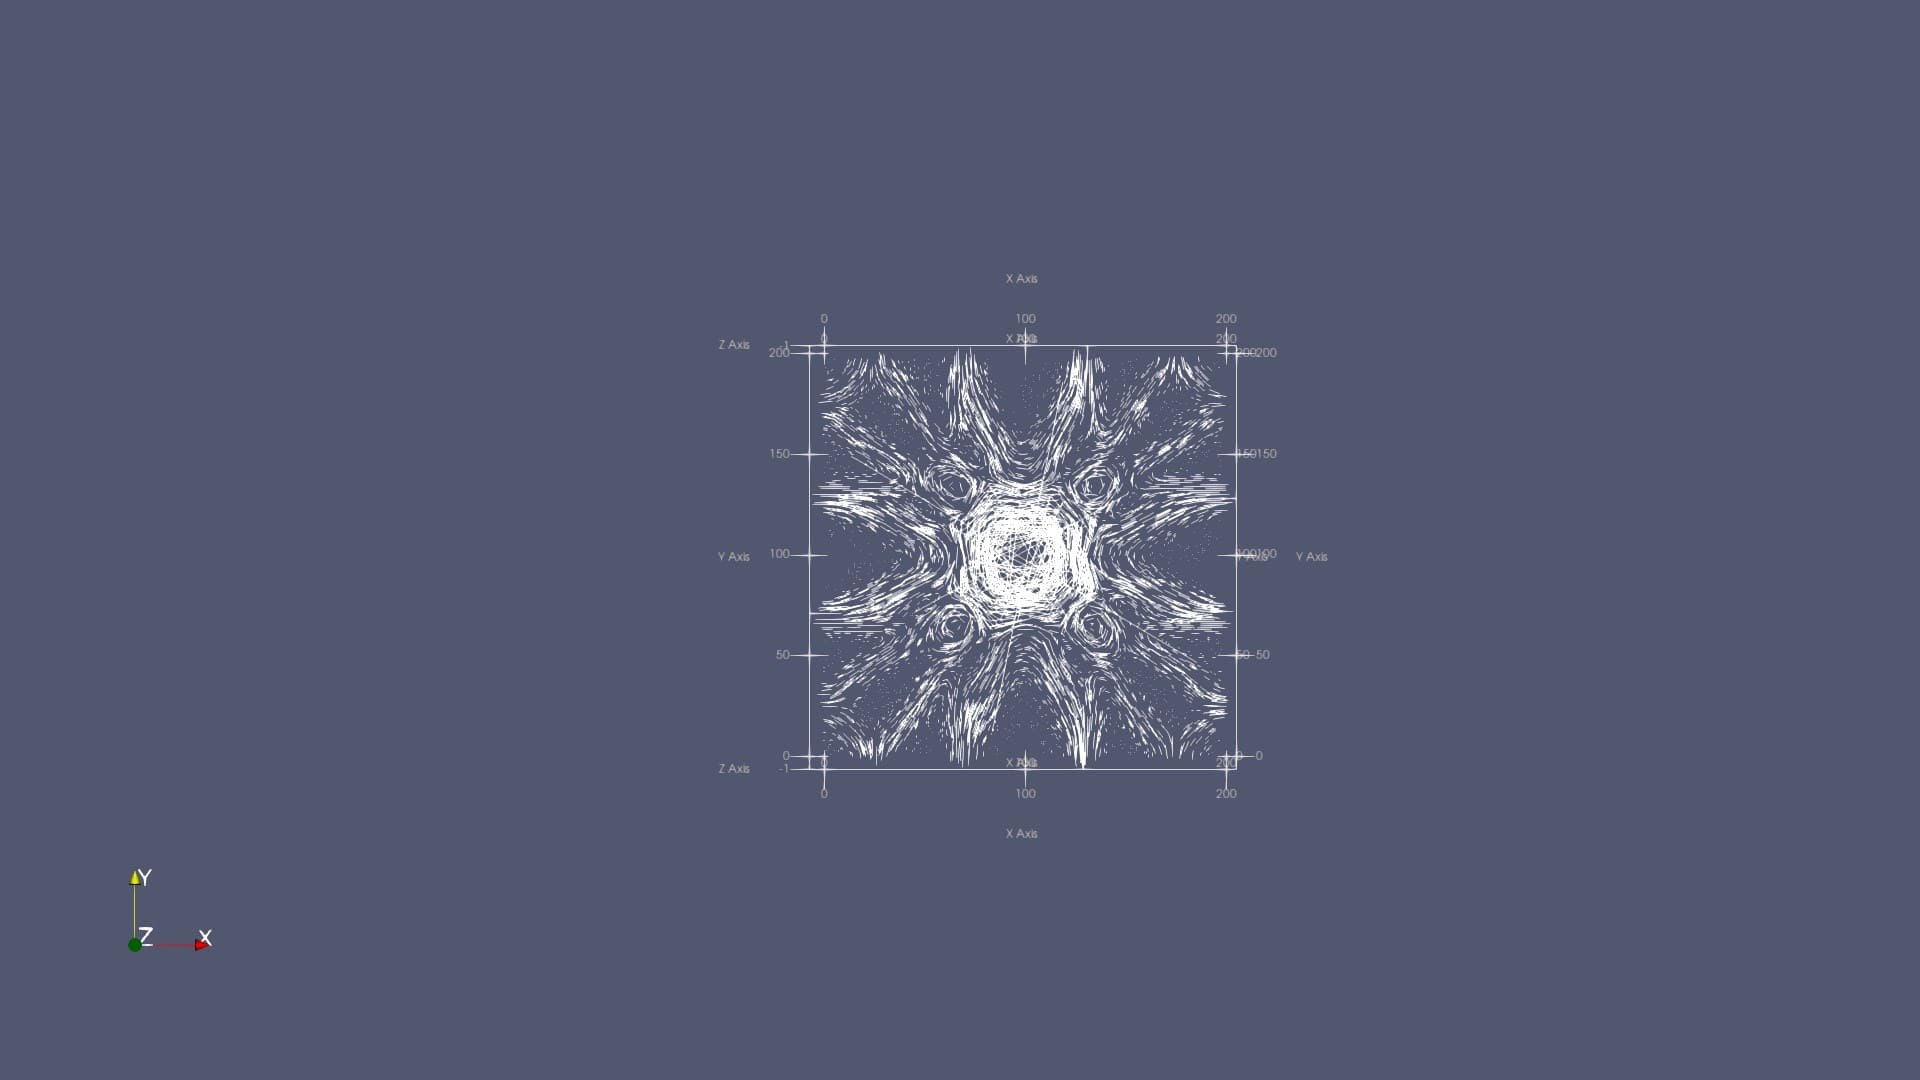
\includegraphics[width=.95\linewidth]{Figures/FDTD2DE3}
    	\caption{t = 600}
    \end{subfigure}
    \begin{subfigure}{.49\textwidth}
    	\centering
    	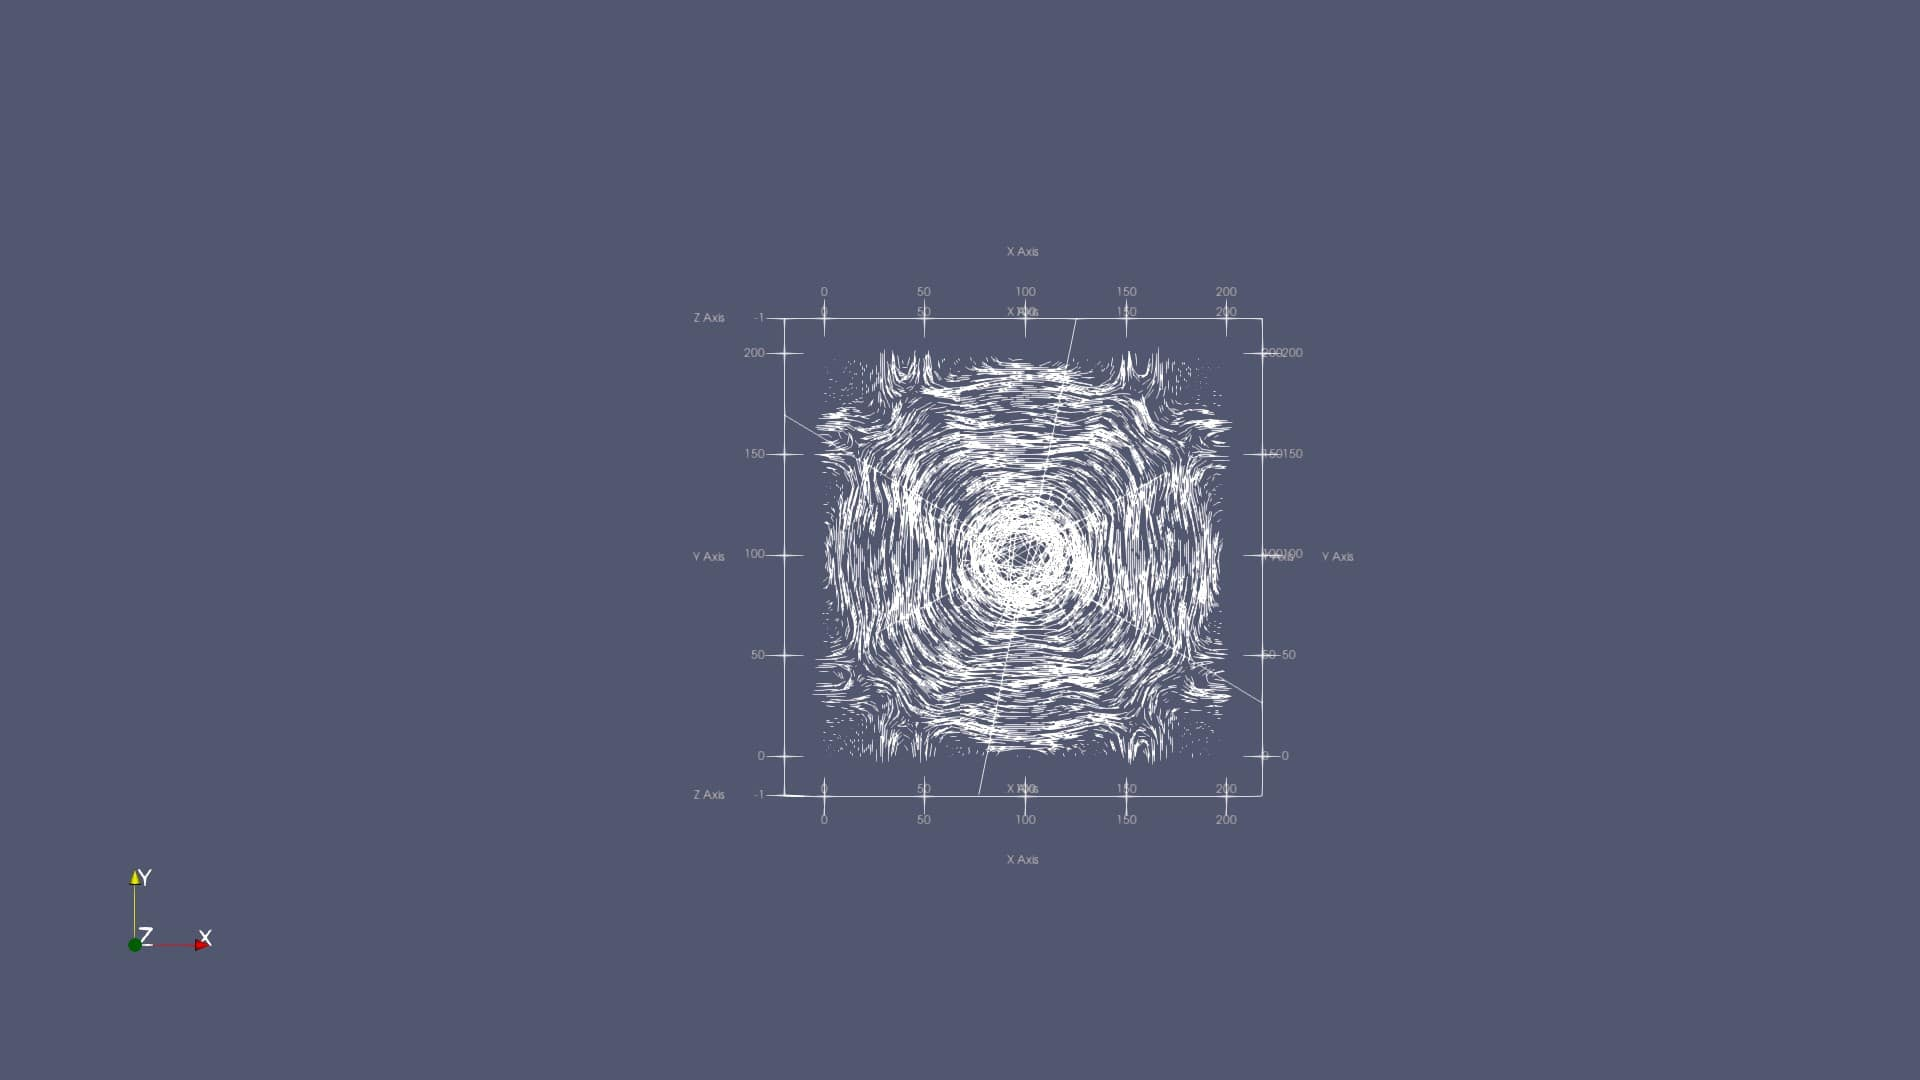
\includegraphics[width=.95\linewidth]{Figures/FDTD2DE4}
    	\caption{t = 800}
    \end{subfigure}
	\decoRule
	\caption[2D Electric Field Simulation]{A simulation of the 2D electric field.}
	\label{fig:FDTD2DE}
\end{figure}

\begin{figure}
	\centering
	\begin{subfigure}{.49\textwidth}
		\centering
		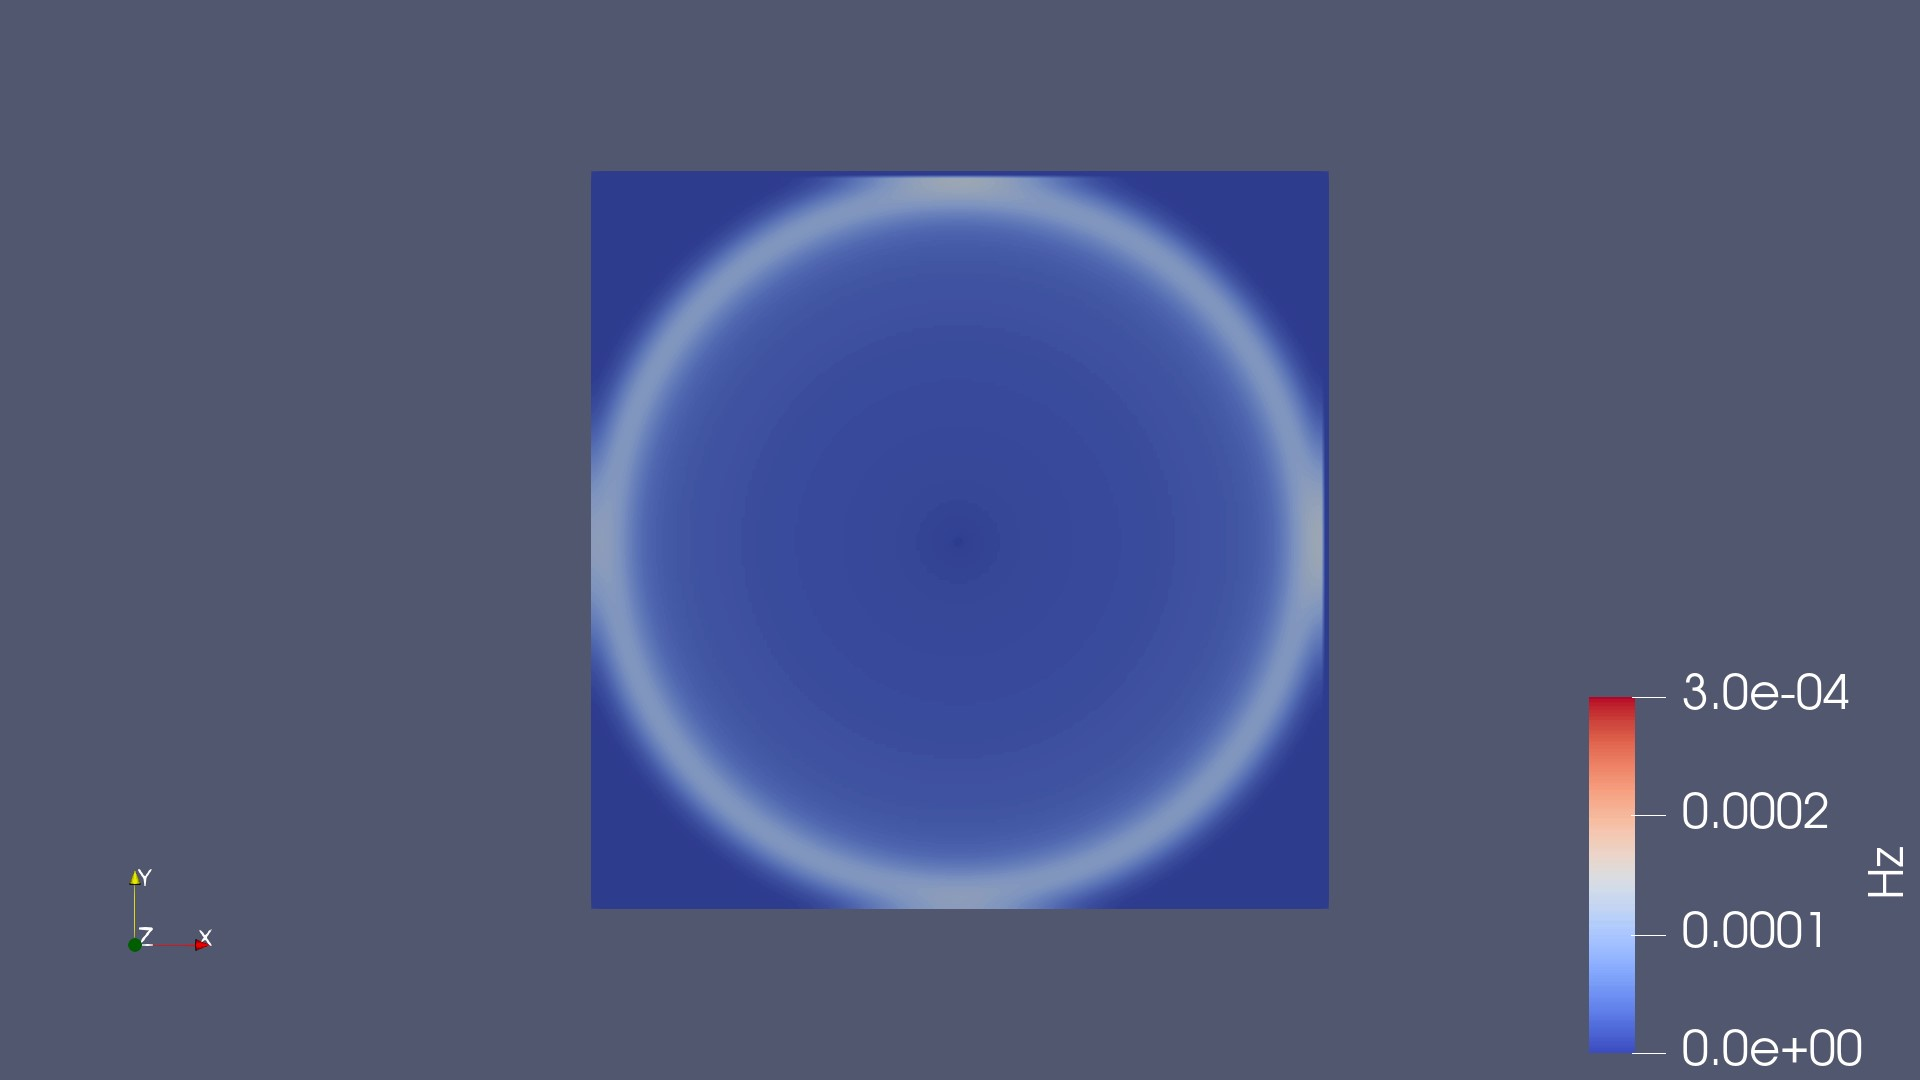
\includegraphics[width=.95\linewidth]{Figures/FDTD2DH1}
		\caption{t = 200}
	\end{subfigure}
	\begin{subfigure}{.49\textwidth}
		\centering
		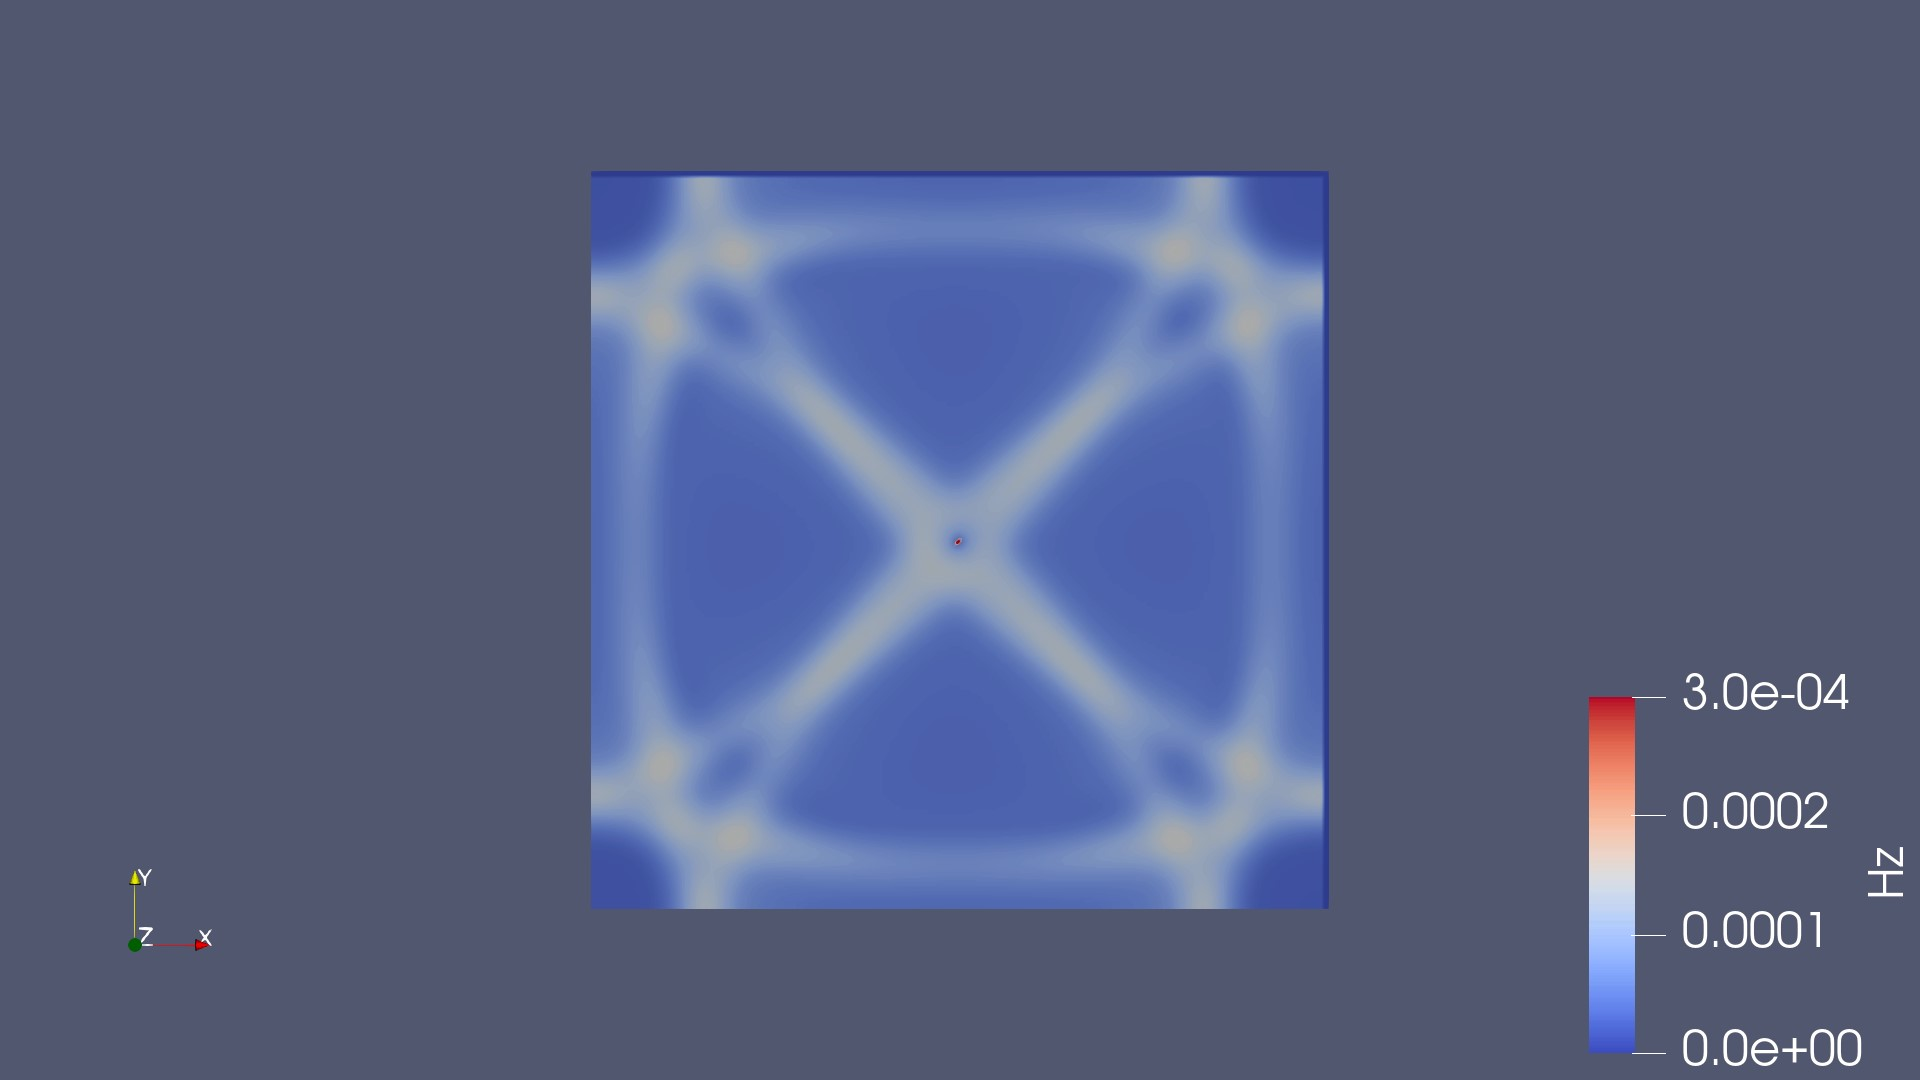
\includegraphics[width=.95\linewidth]{Figures/FDTD2DH2}
		\caption{t = 400}
	\end{subfigure}
	\begin{subfigure}{.49\textwidth}
		\centering
		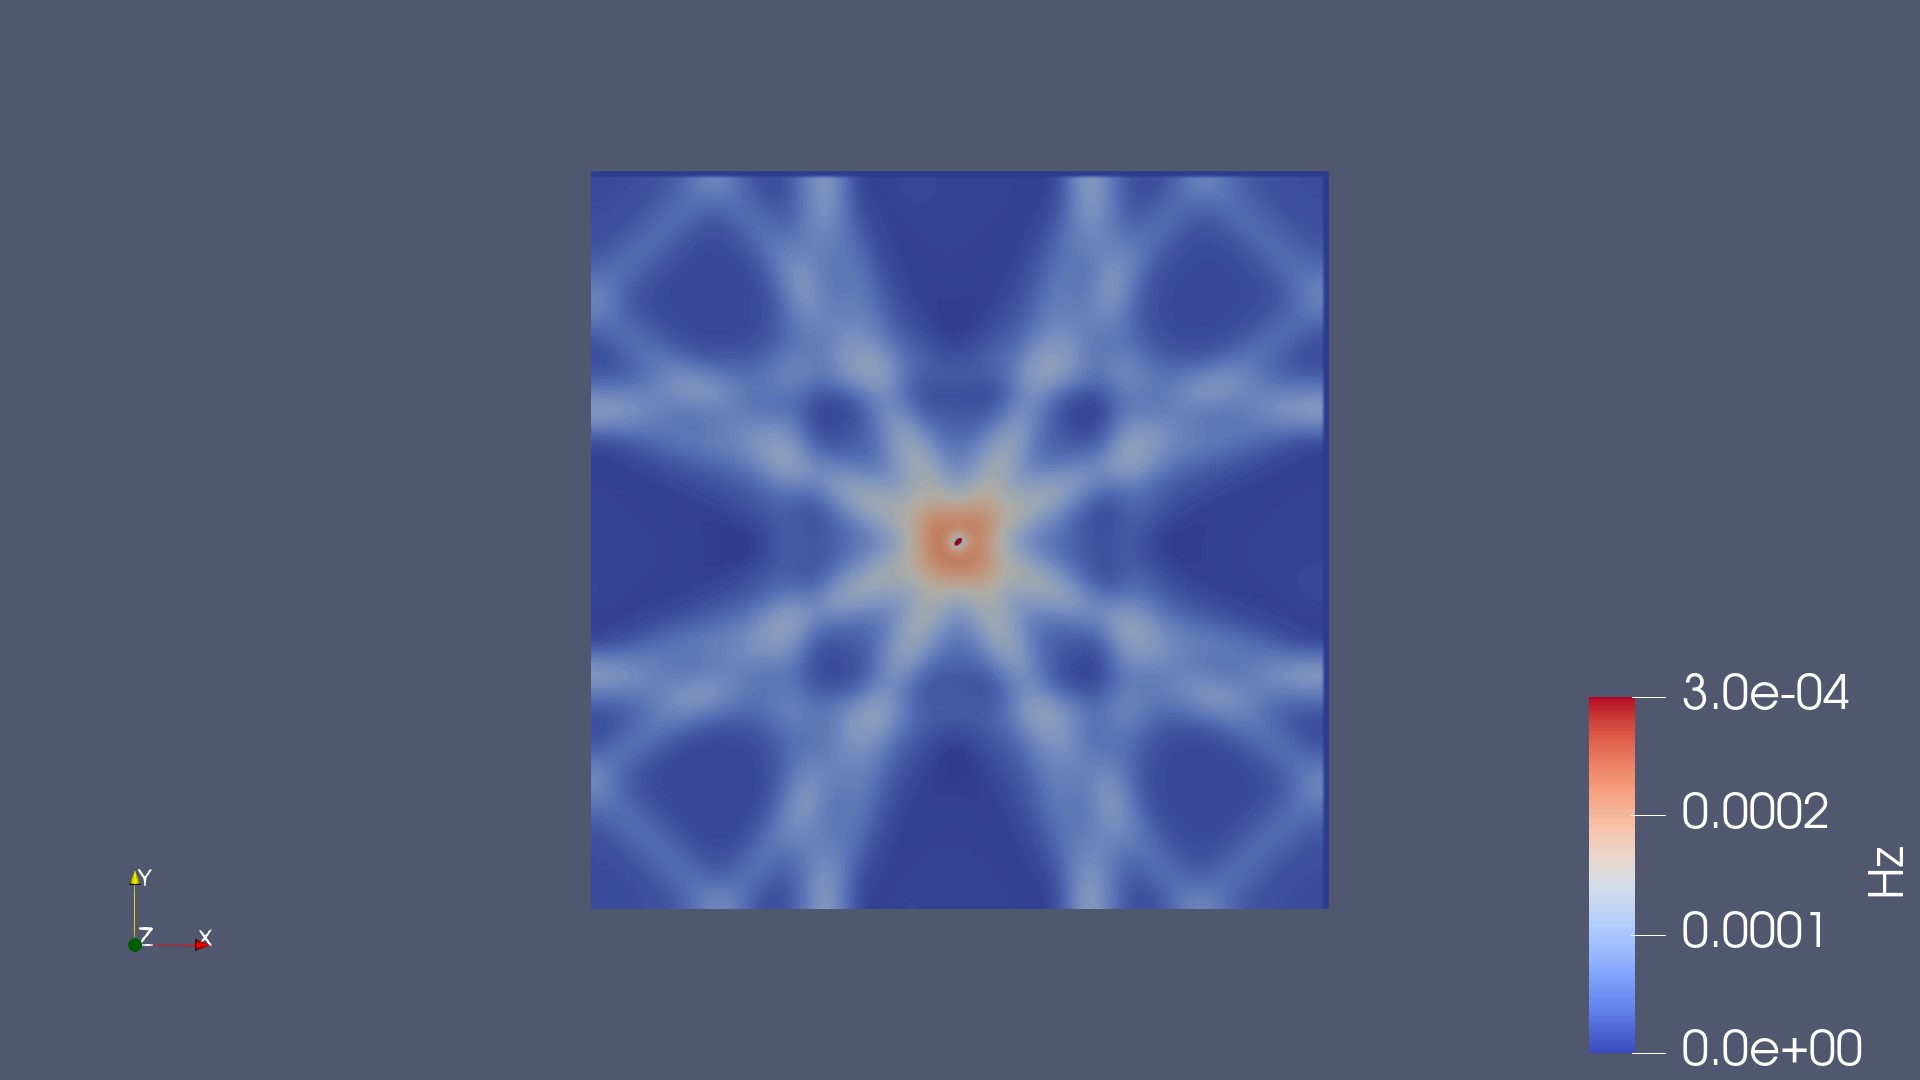
\includegraphics[width=.95\linewidth]{Figures/FDTD2DH3}
		\caption{t = 600}
	\end{subfigure}
	\begin{subfigure}{.49\textwidth}
		\centering
		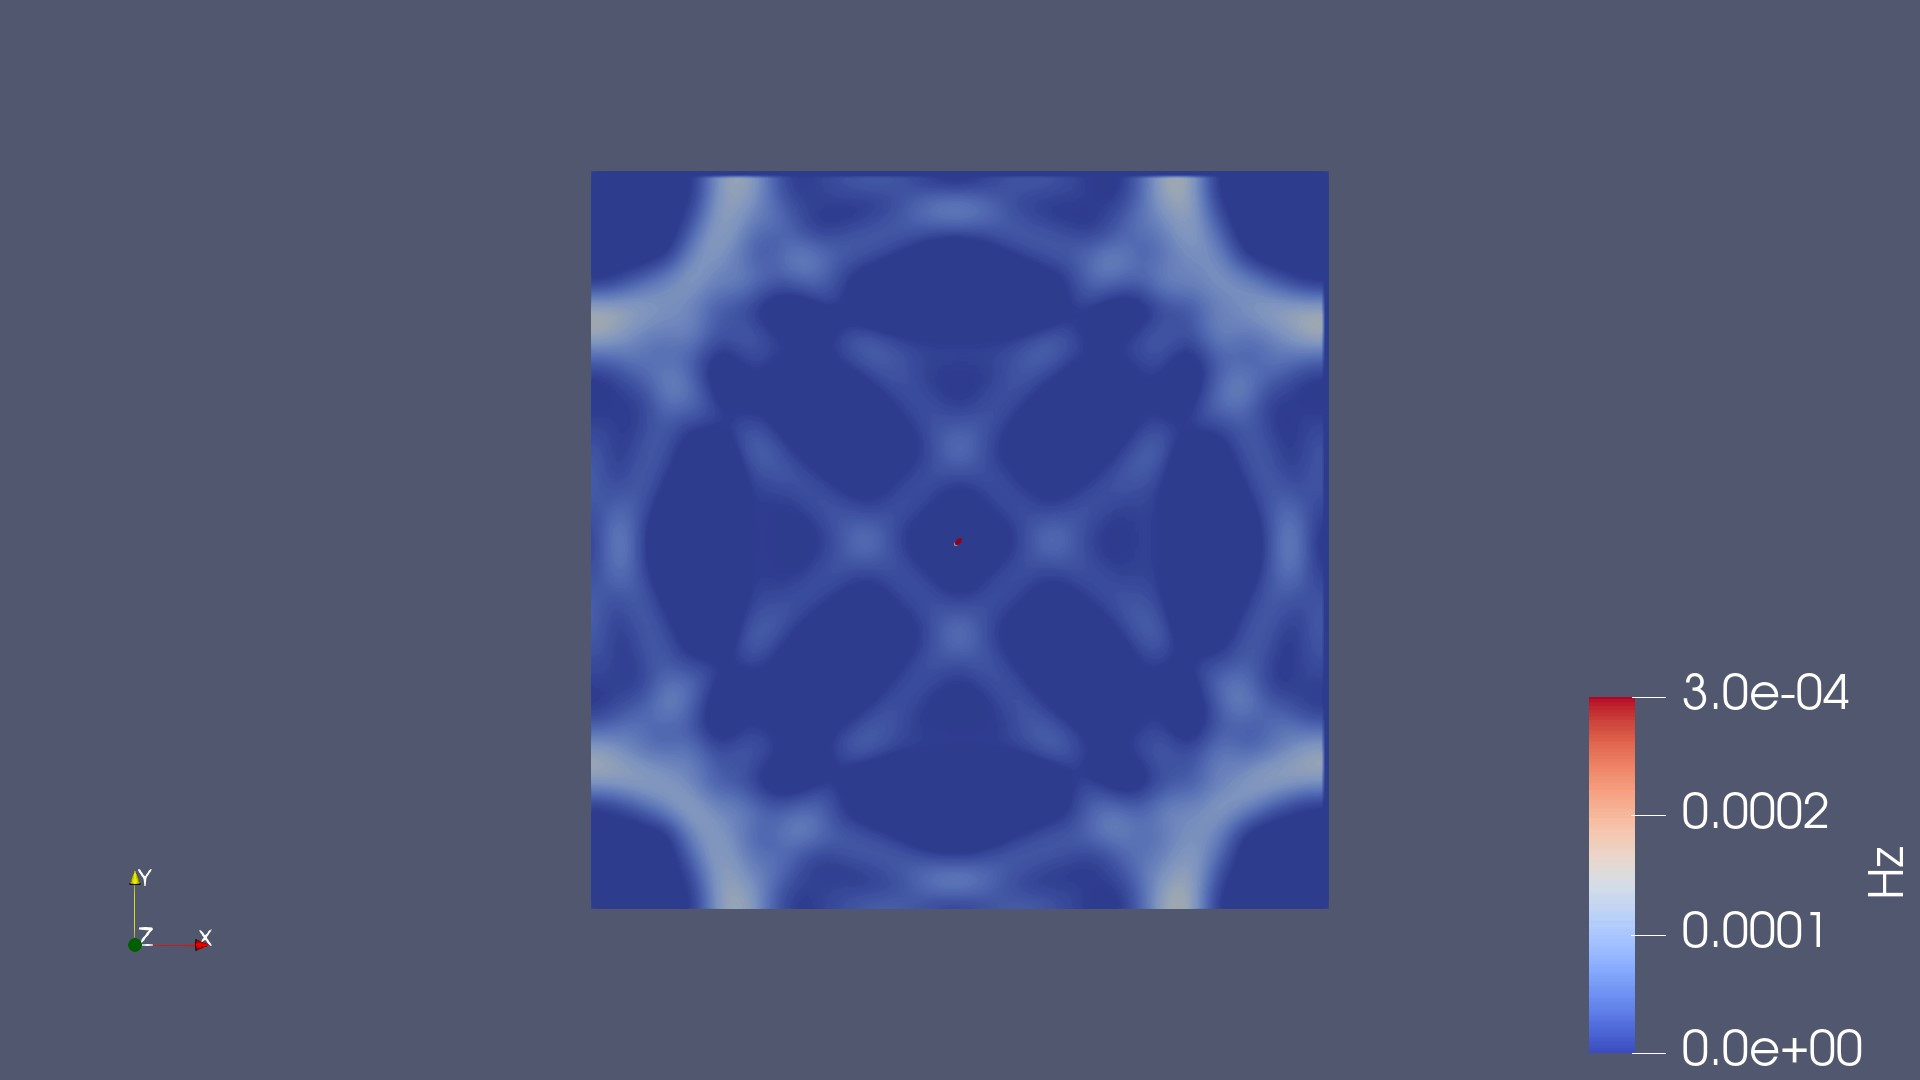
\includegraphics[width=.95\linewidth]{Figures/FDTD2DH4}
		\caption{t = 800}
	\end{subfigure}
	\decoRule
	\caption[2D Magnetic Field Simulation]{A simulation of the 2D magnetic field.}
	\label{fig:FDTD2DH}
\end{figure}